\begin{frame}\frametitle {Real-$\gamma$ Background}

Main sources of true $\gamma$ background are $Z\gamma$ and $W\gamma \rightarrow \tau \nu \gamma$. The MC-based estimation is used to subtract these backgrounds.

MC-based background estimation.

\end{frame}%{Real-$\gamma$ Backgrounds}

\begin{frame}\frametitle{\footnotesize{$P_T^{\gamma}$ Spectrum before and after Background Subtraction. Muon Channel, Barrel}}
  \tiny{Top: data vs fake-$\gamma$ background derived from the template method + real-$\gamma$ background predicted by dedicated MC samples + signal MC, with $I_{ch}$ and $\sigma_{i\eta{i}\eta}$ used as fit variables. Bottom: left: data yields after full background subtraction vs signal MC. $I_{ch}$ vs $\sigma_{i\eta{i}\eta}$ fit results. Right: fake-$\gamma$ data driven background prediction vs MC. Plotted with the stat error only. Disagreement}
  \begin{figure}[htb]
    \begin{center}
       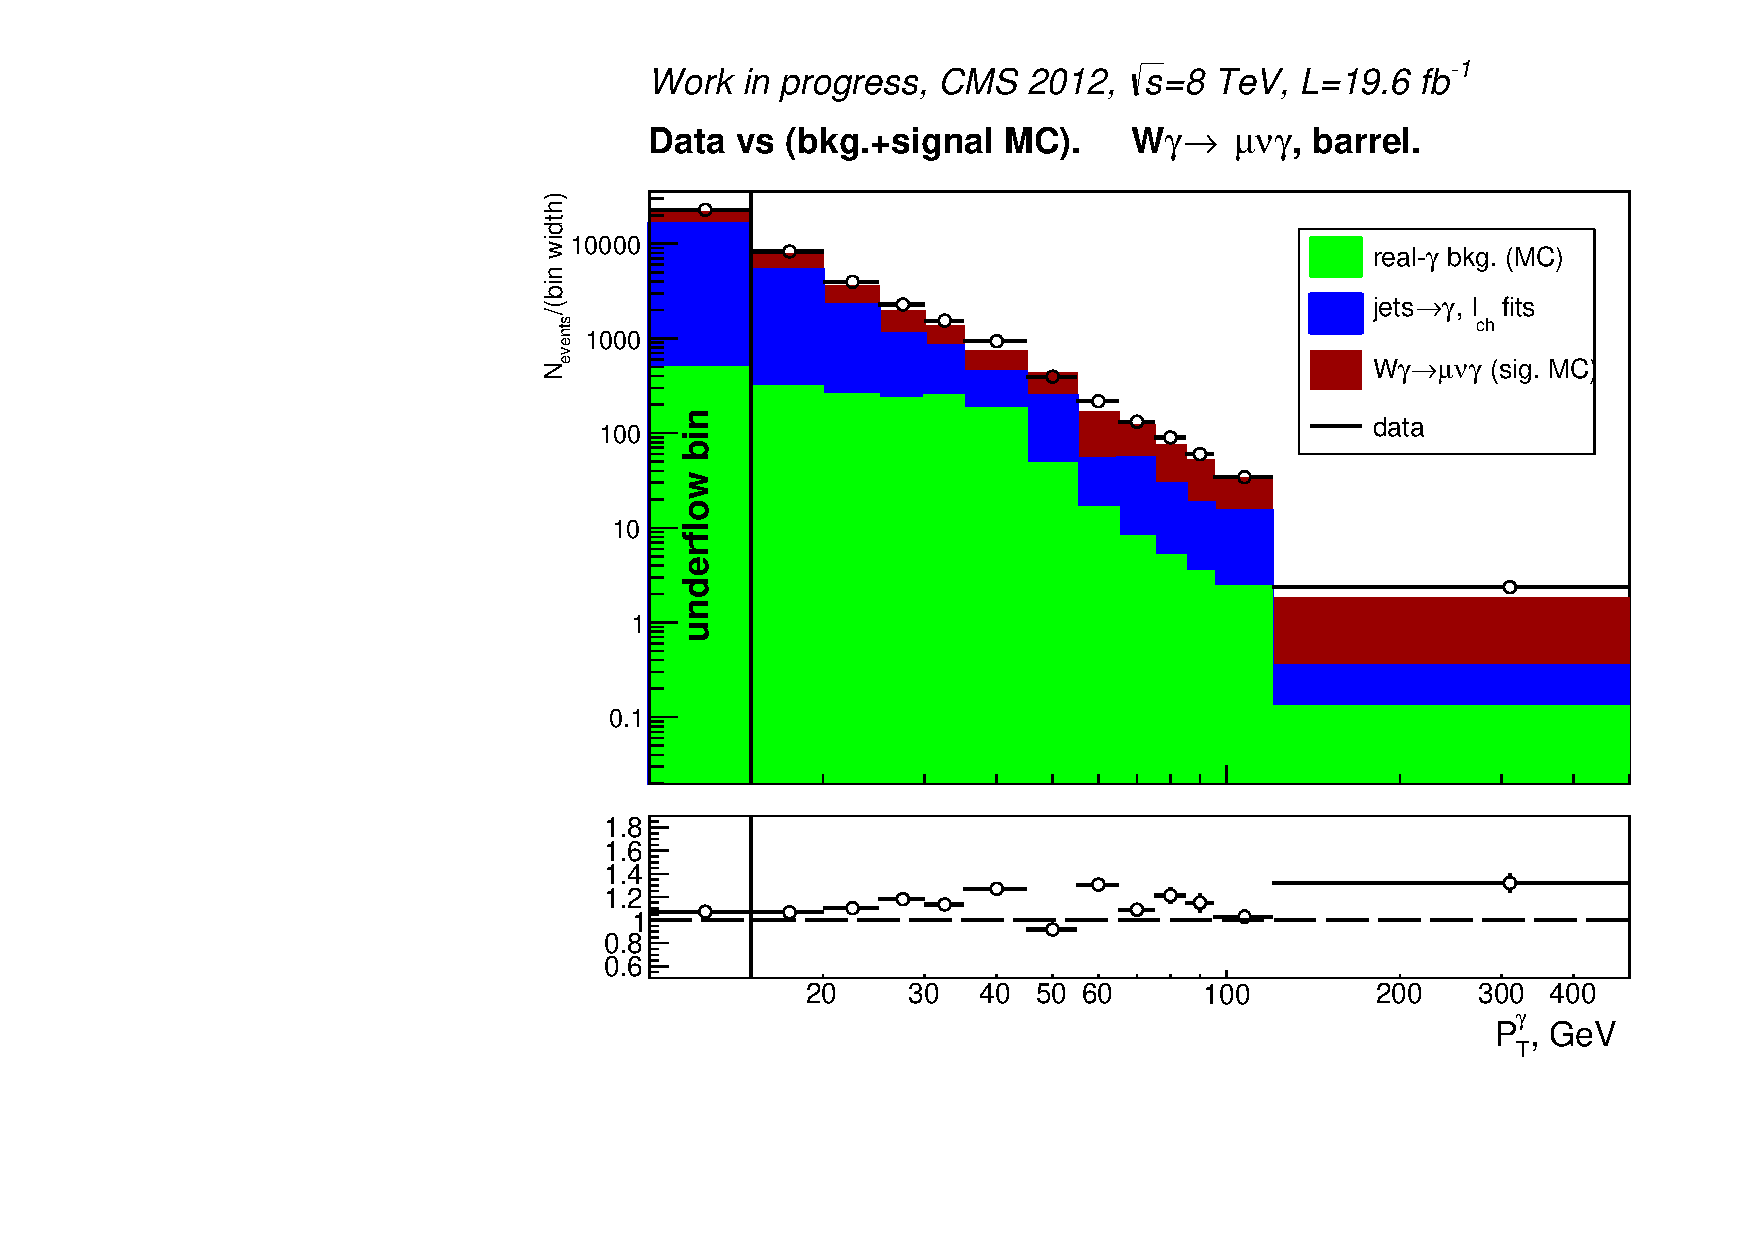
\includegraphics[width=0.25\textwidth]{../figs/figs_v11/MUON_WGamma/PrepareYields/c_DATAvsBkgPlusSigMCc_MUON_WGamma_TEMPL_CHISO_UNblind__Barrel__phoEt.pdf}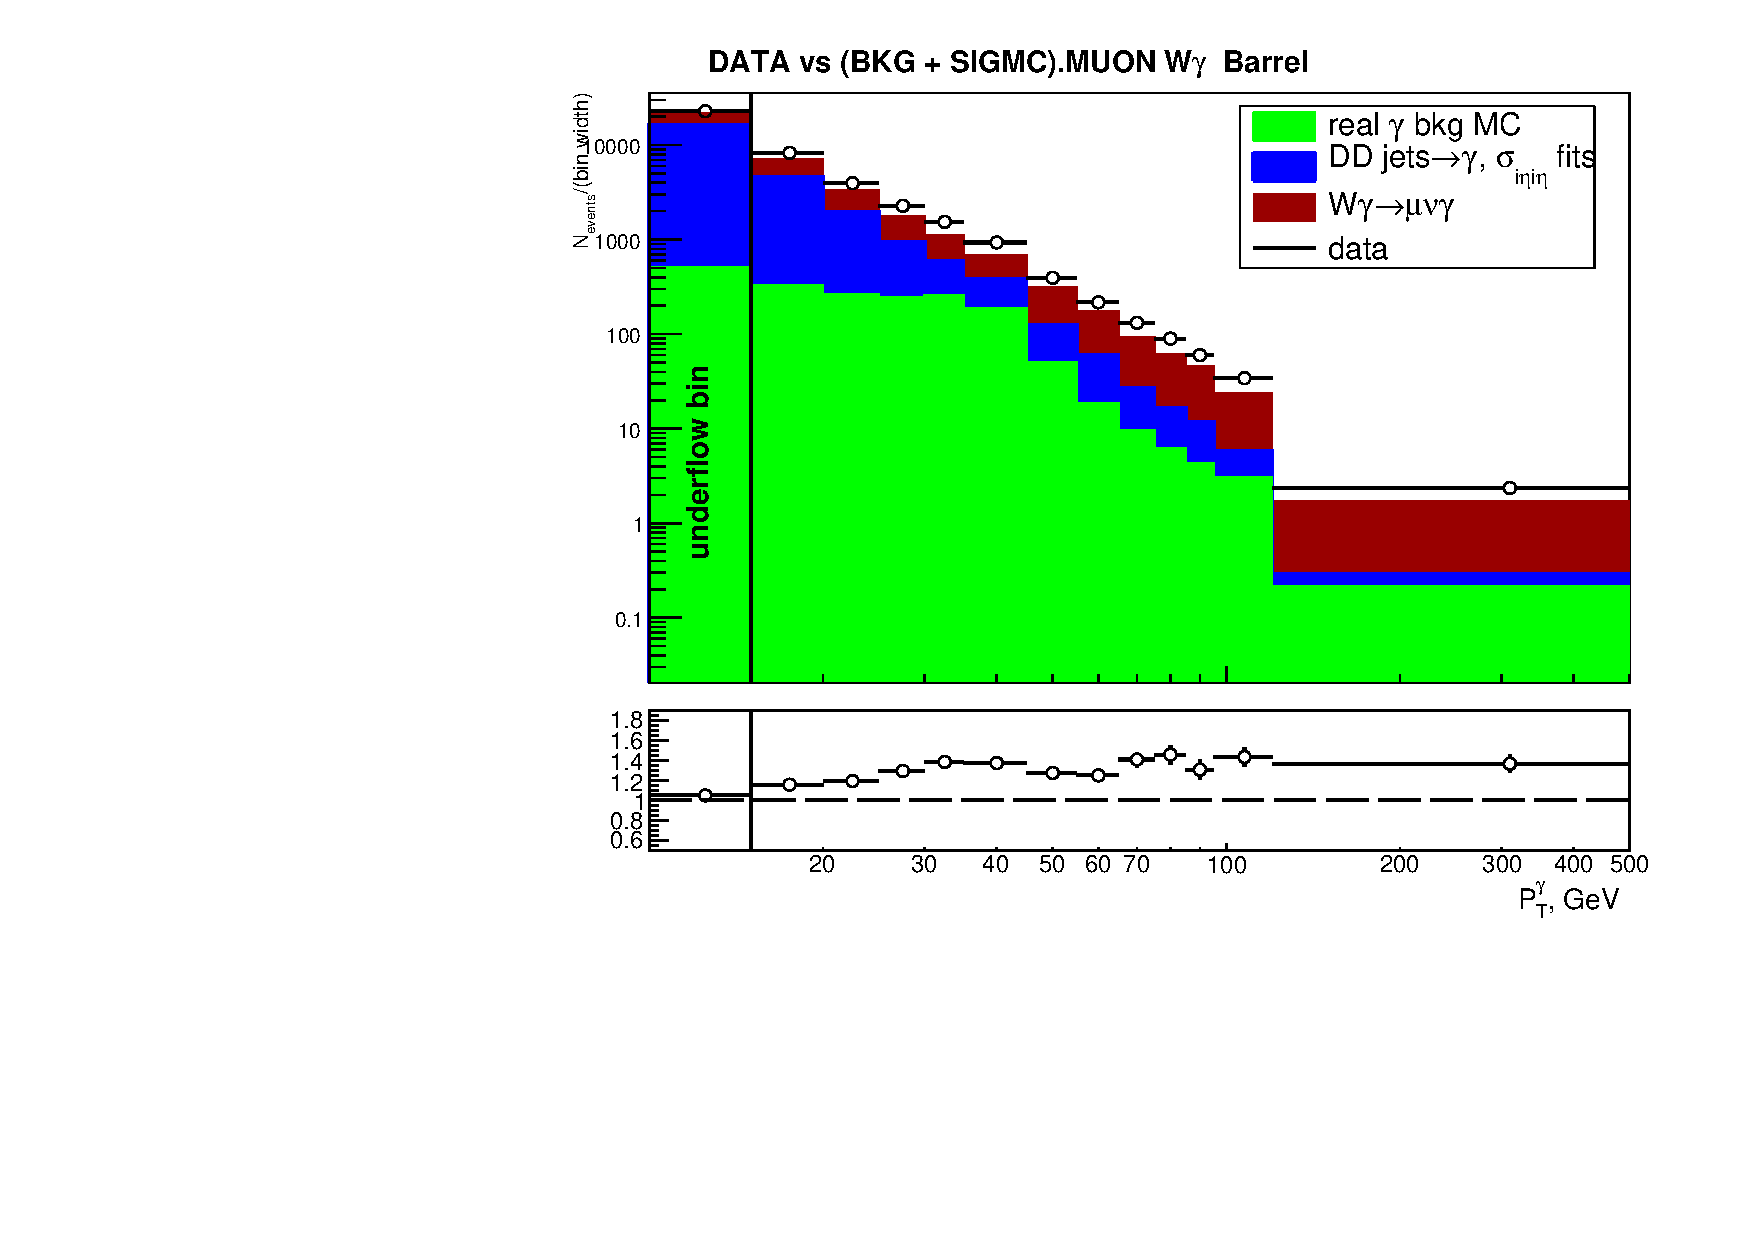
\includegraphics[width=0.25\textwidth]{../figs/figs_v11/MUON_WGamma/PrepareYields/c_DATAvsBkgPlusSigMCc_MUON_WGamma_TEMPL_SIHIH_UNblind__Barrel__phoEt.pdf}\\
       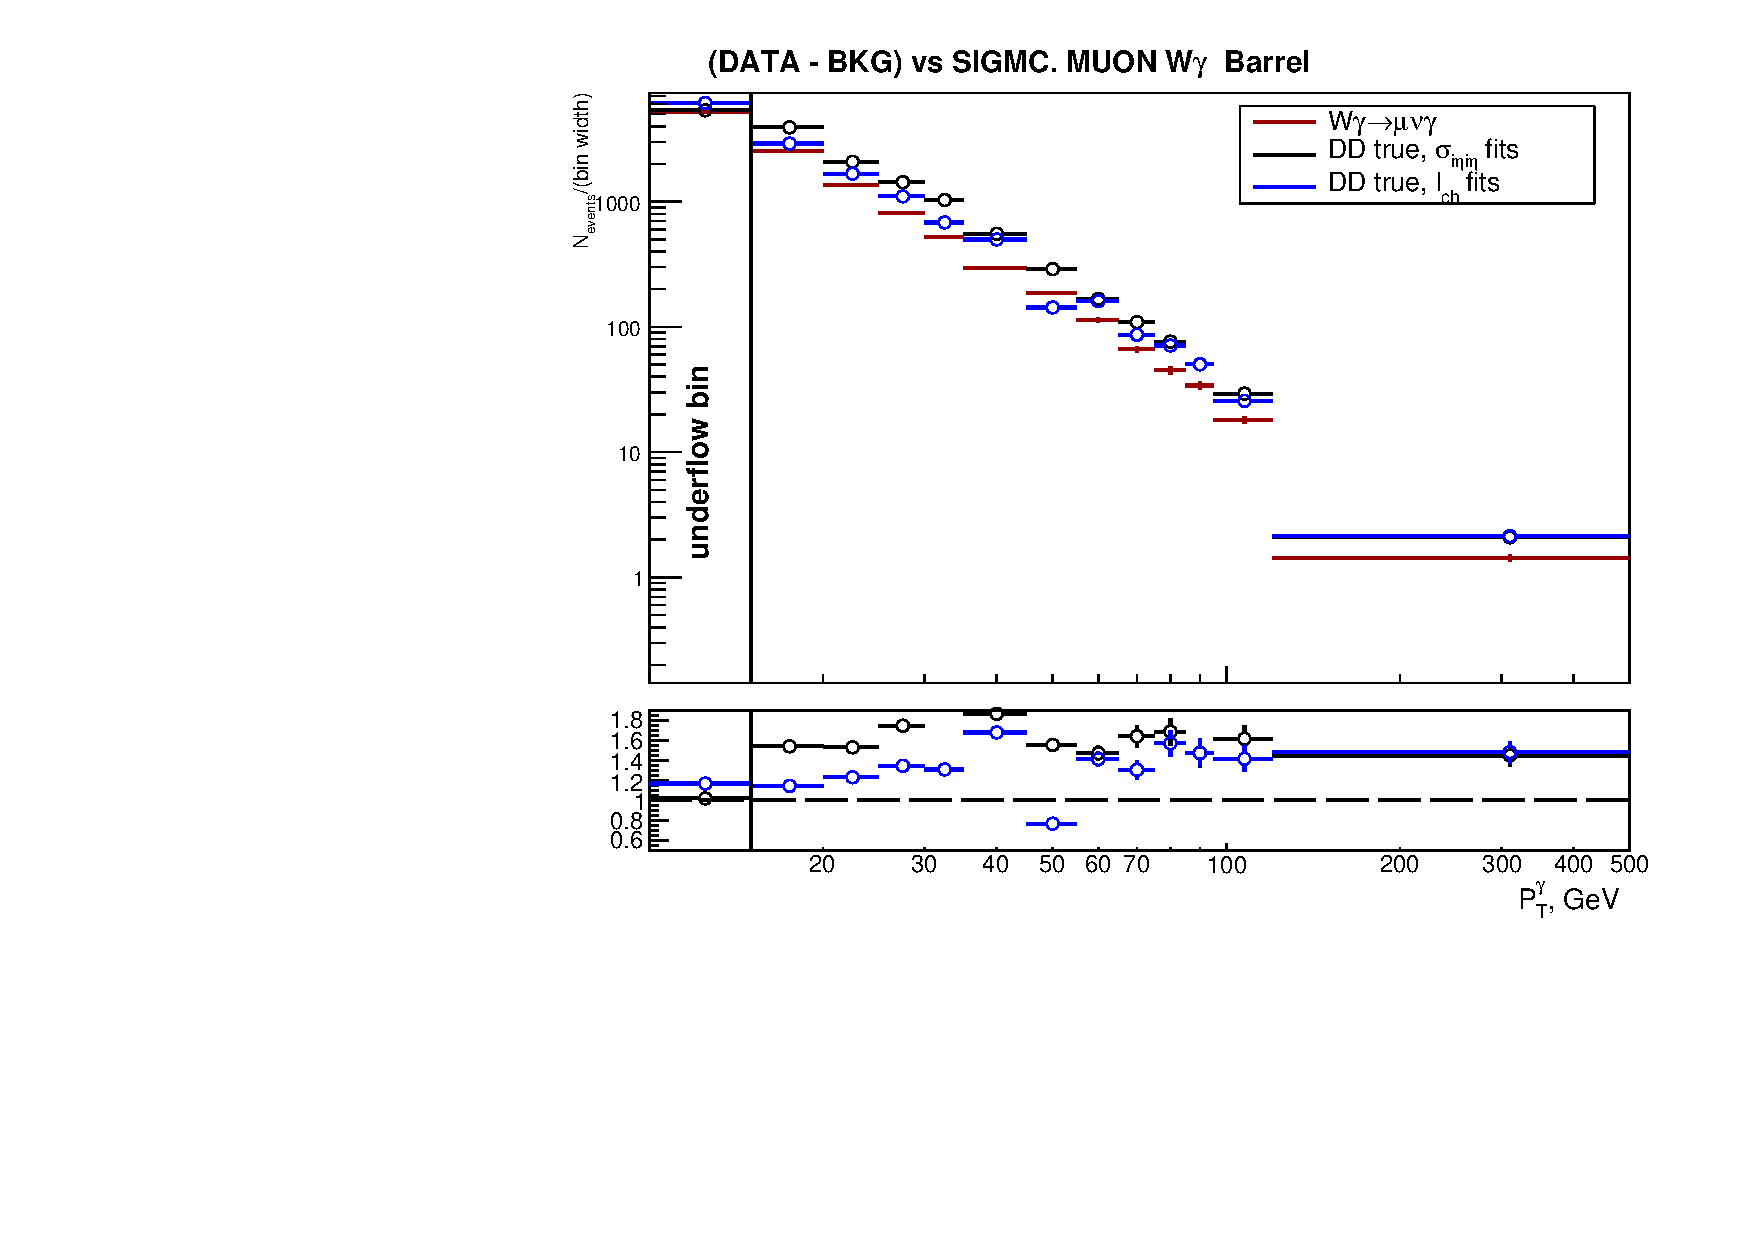
\includegraphics[width=0.25\textwidth]{../figs/figs_v11/MUON_WGamma/PrepareYields/c_BkgSubtrDATAvsSIGMC_c_MUON_WGamma__UNblind__Barrel__phoEt.pdf}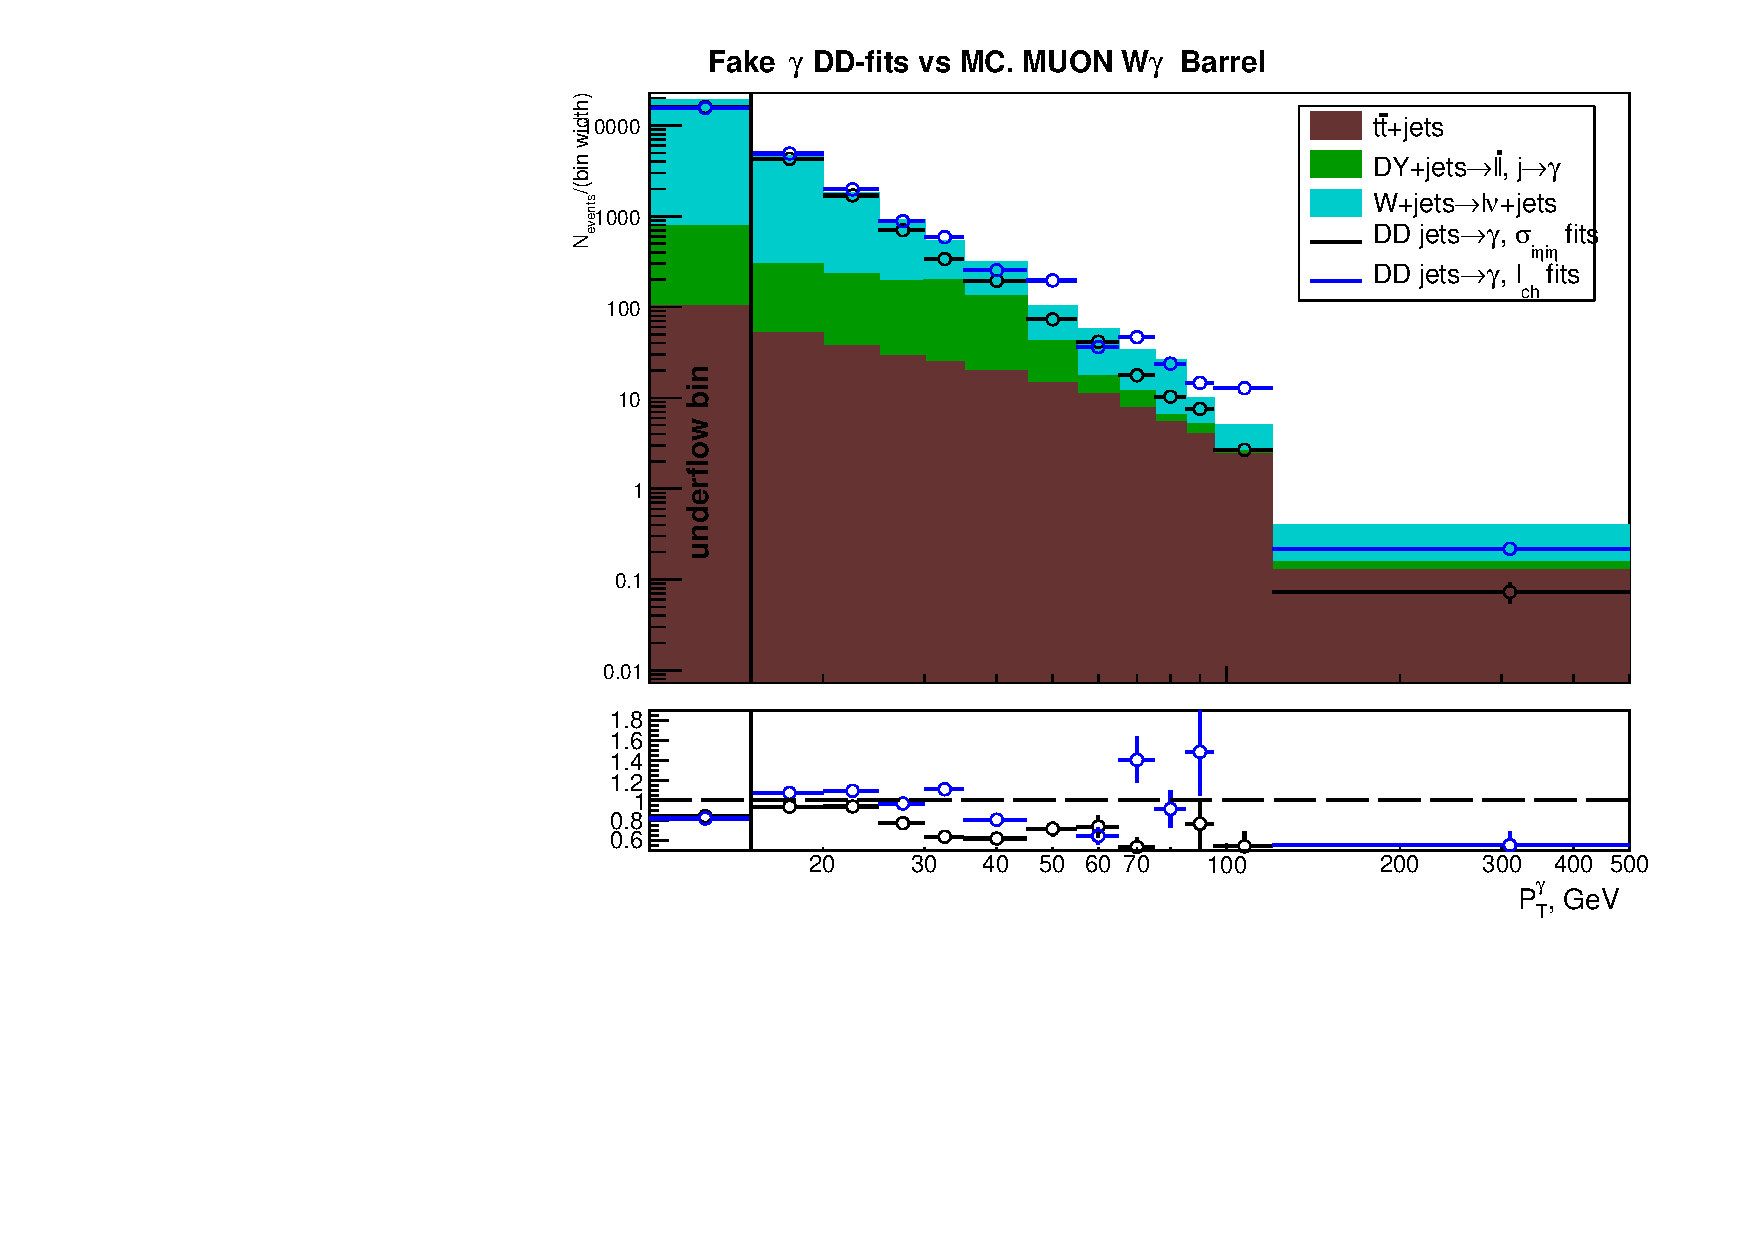
\includegraphics[width=0.25\textwidth]{../figs/figs_v11/MUON_WGamma/PrepareYields/c_FakeDDvsMC_c_MUON_WGamma__UNblind__Barrel__phoEt.pdf}\\
    \end{center}
  \end{figure}
\end{frame}%{$jets \rightarrow \gamma$ Background Subtraction. Plots, W$\gamma$}

\begin{frame}\frametitle{\footnotesize{$P_T^{\gamma}$ Spectrum before and after Background Subtraction. Electron Channel, Barrel}}
  \tiny{Top: data vs fake-$\gamma$ background derived from the template method + real-$\gamma$ background predicted by dedicated MC samples + signal MC, with $I_{ch}$ and $\sigma_{i\eta{i}\eta}$ used as fit variables. Bottom: left: data yields after full background subtraction vs signal MC. $I_{ch}$ vs $\sigma_{i\eta{i}\eta}$ fit results. Right: fake-$\gamma$ data driven background prediction vs MC. Plotted with the stat error only.}
  \begin{figure}[htb]
    \begin{center}
       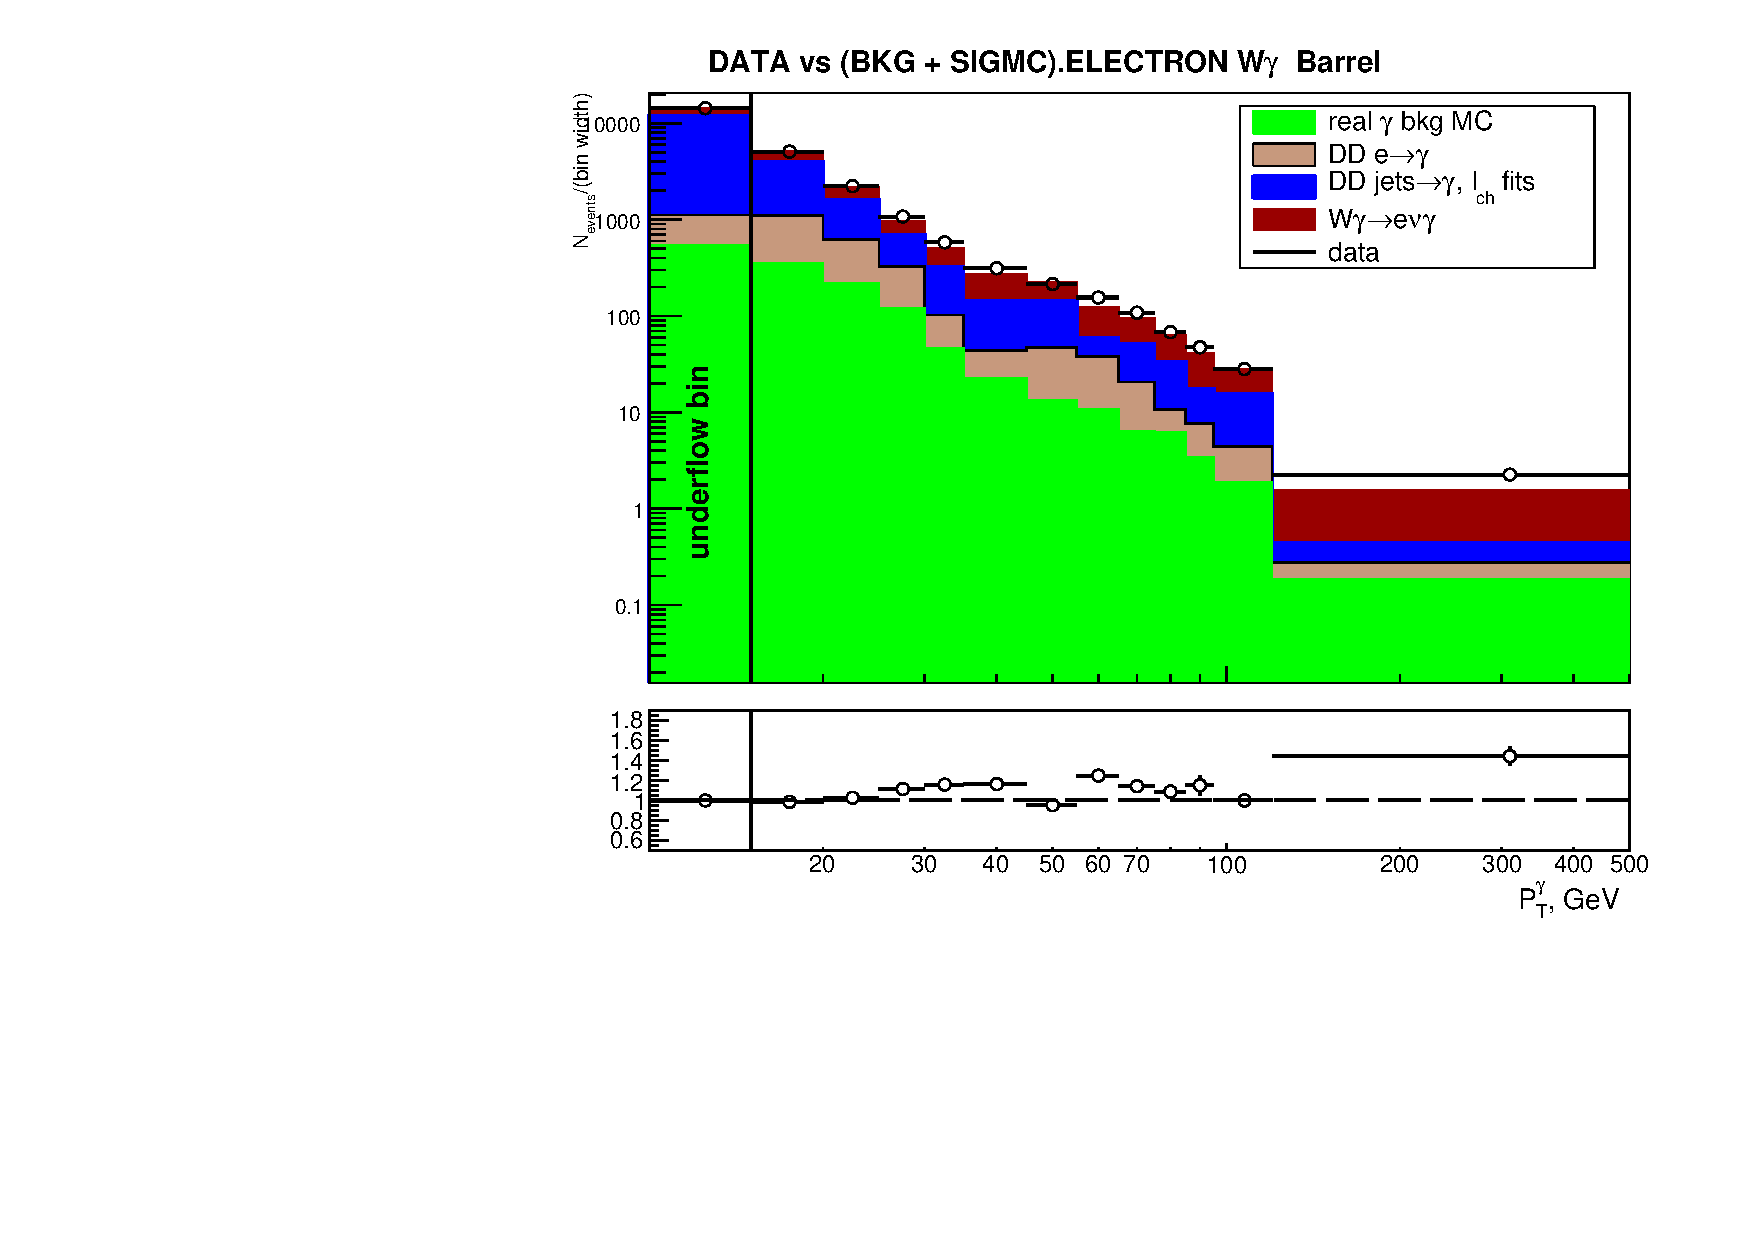
\includegraphics[width=0.25\textwidth]{../figs/figs_v11/ELECTRON_WGamma/PrepareYields/c_DATAvsBkgPlusSigMCc_ELECTRON_WGamma_TEMPL_CHISO_UNblind__Barrel__phoEt.pdf}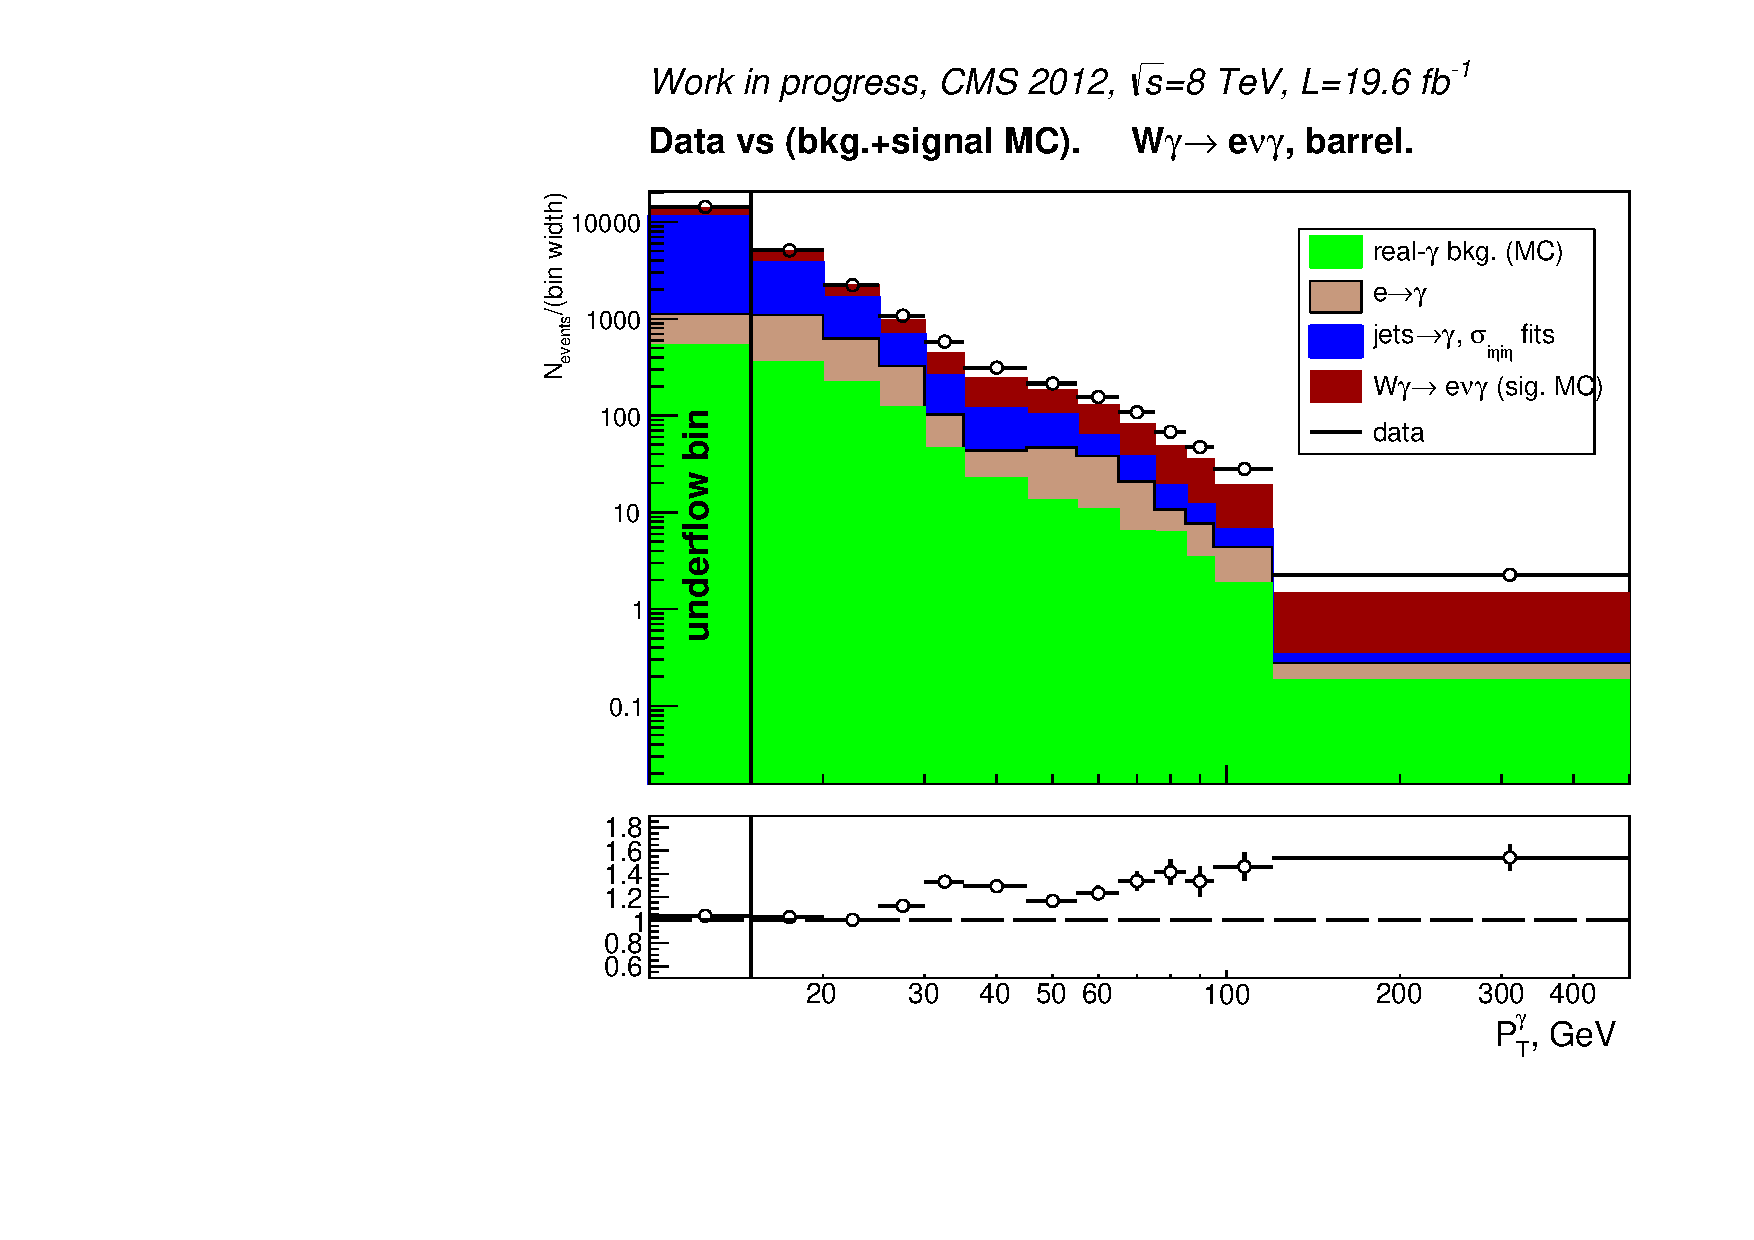
\includegraphics[width=0.25\textwidth]{../figs/figs_v11/ELECTRON_WGamma/PrepareYields/c_DATAvsBkgPlusSigMCc_ELECTRON_WGamma_TEMPL_SIHIH_UNblind__Barrel__phoEt.pdf}\\
       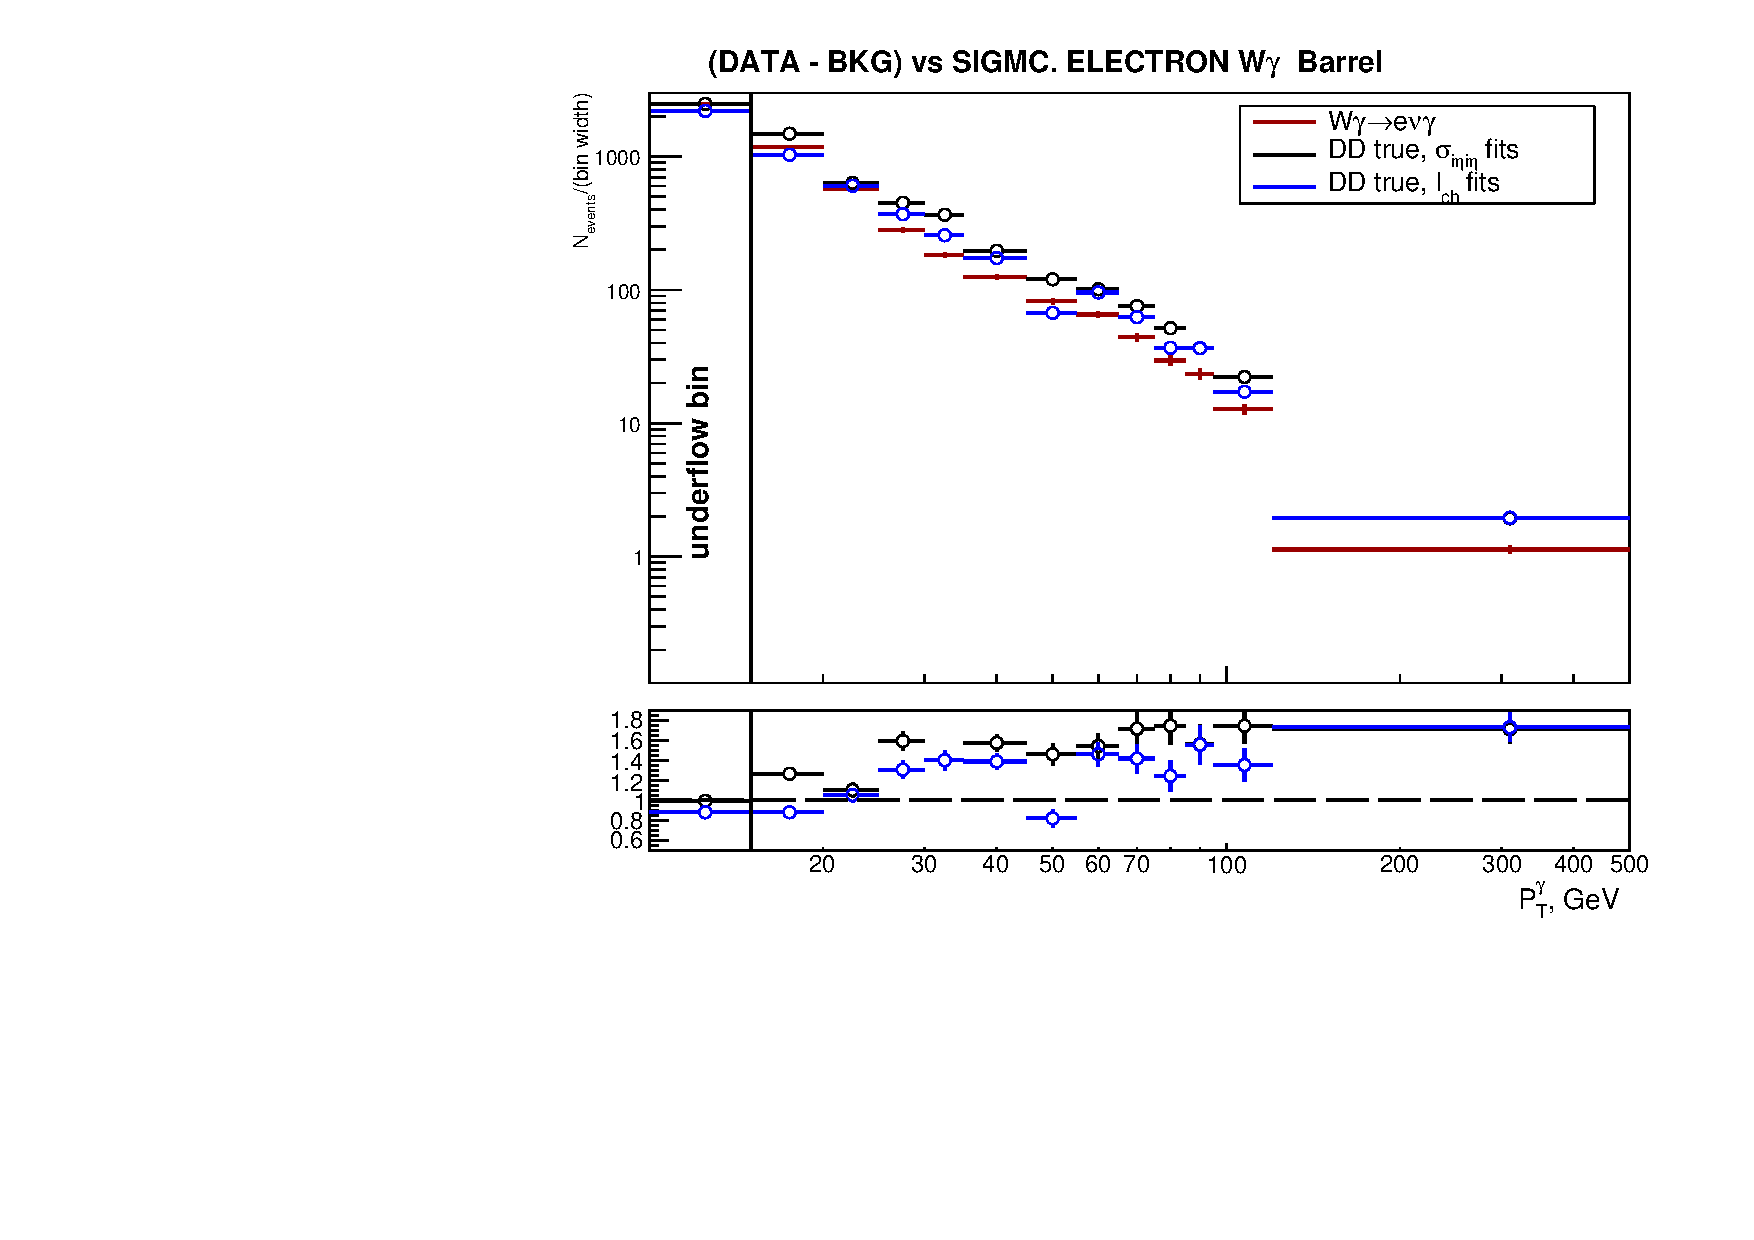
\includegraphics[width=0.25\textwidth]{../figs/figs_v11/ELECTRON_WGamma/PrepareYields/c_BkgSubtrDATAvsSIGMC_c_ELECTRON_WGamma__UNblind__Barrel__phoEt.pdf}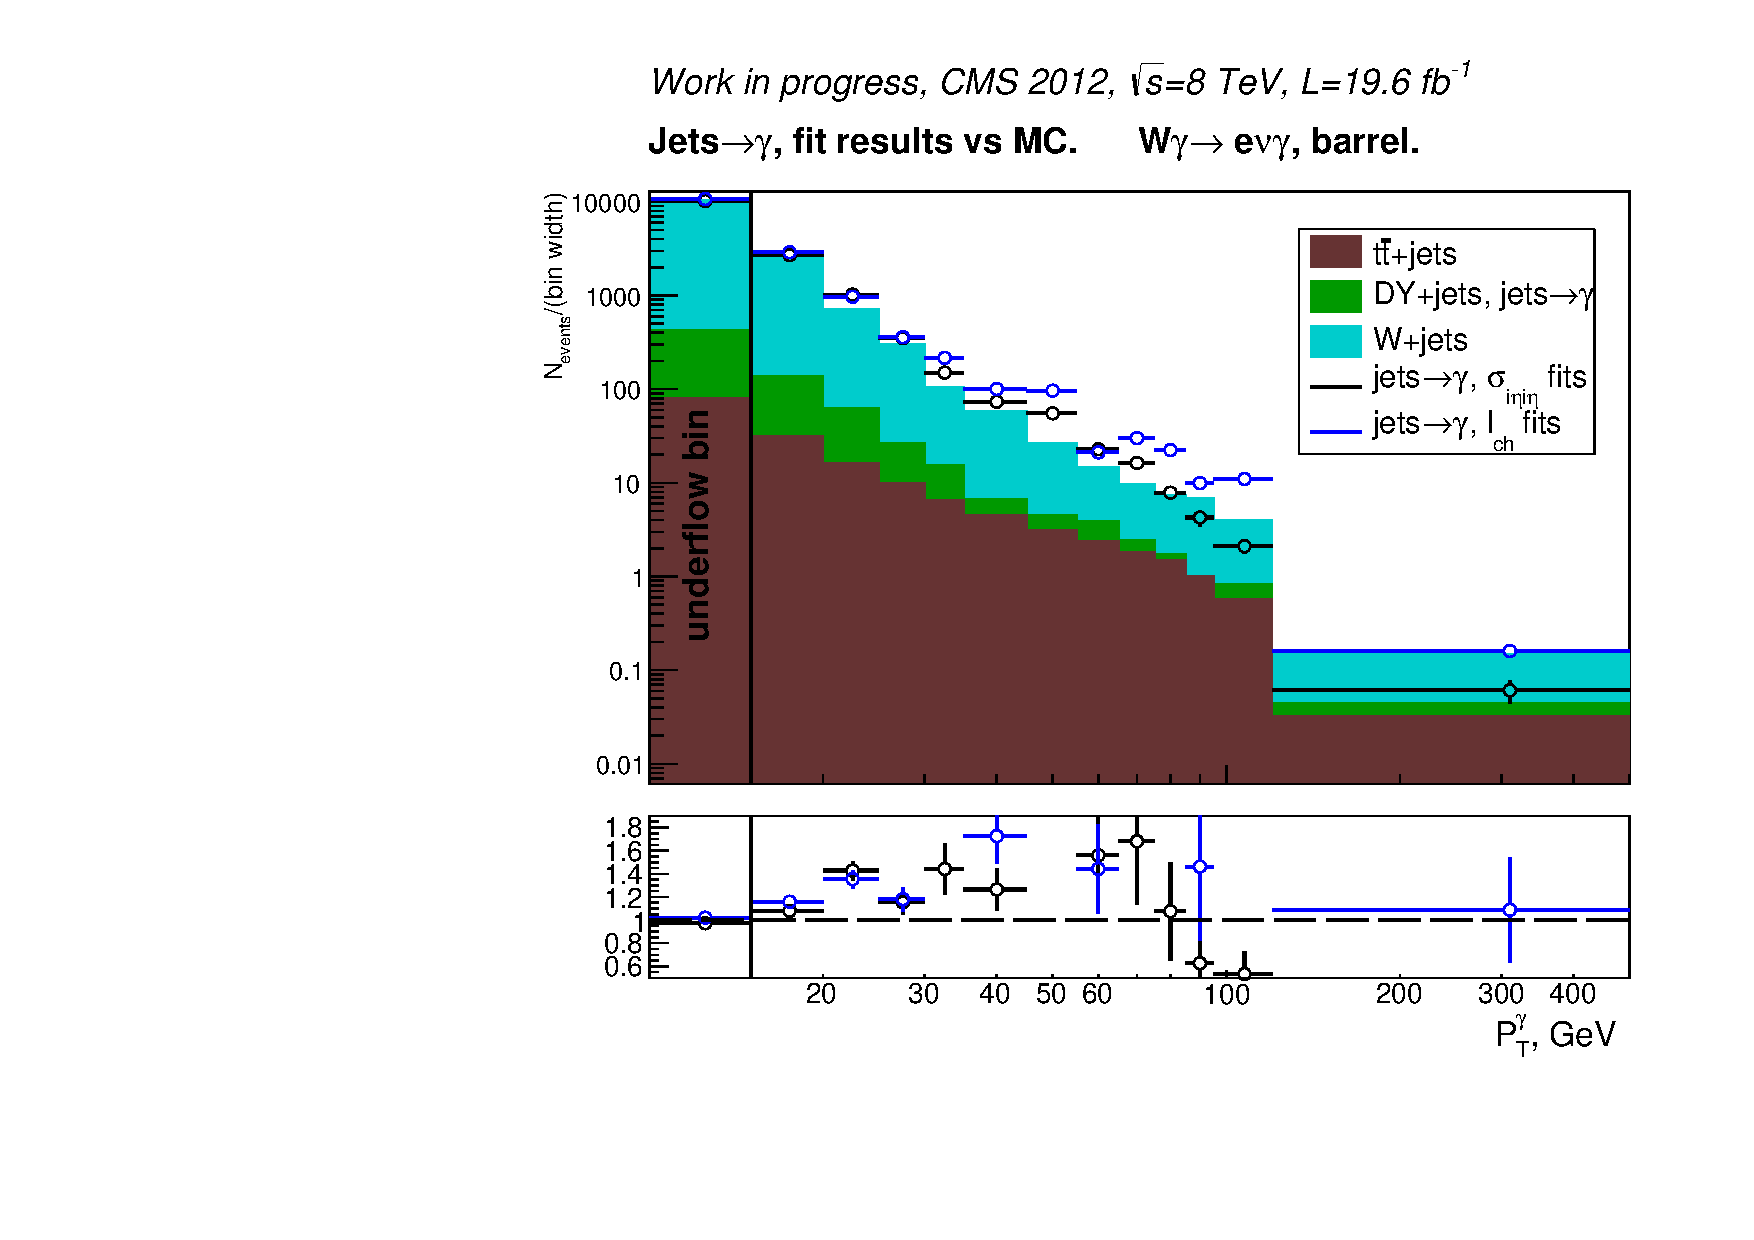
\includegraphics[width=0.25\textwidth]{../figs/figs_v11/ELECTRON_WGamma/PrepareYields/c_FakeDDvsMC_c_ELECTRON_WGamma__UNblind__Barrel__phoEt.pdf}\\
    \end{center}
  \end{figure}
\end{frame}%{$jets \rightarrow \gamma$ Background Subtraction. Plots, W$\gamma$}

\begin{frame}\frametitle {Cross Checks for Jets$\rightarrow\gamma$ Background Estimation}

\footnotesize{\bfseries{Simple MC closure check:}}\scriptsize{}

\footnotesize{\bfseries{MC realistic check:}}\scriptsize{}

\footnotesize{\bfseries{$Z\gamma$ check:}}\scriptsize{}

\footnotesize{\bfseries{Conclusions:}}\scriptsize{}

\end{frame}%{Real-$\gamma$ Backgrounds}
